\marginnote{\href{https://youtu.be/3eiio3Tw7UQ}{Video}}
\marginnote{\href{https://ocw.mit.edu/courses/6-041sc-probabilistic-systems-analysis-and-applied-probability-fall-2013/pages/unit-iv/lecture-19/}{Lecture Home}}
\marginnote{\href{https://ocw.mit.edu/courses/6-041sc-probabilistic-systems-analysis-and-applied-probability-fall-2013/d569abb143b22f469a09ff218cb3383c_MIT6_041SCF13_L19.pdf}{Slides}}
Reading: 5.1-5.3, Start 5.4
\\
Introducing limit theorems\\

Collect n samples:  $X_1,\ldots, X_n$, iid.

This is the estimate of your expected value:
\begin{align*}
    M_n = \frac{X_1 +\cdots + X_n}{n}, \qquad \text{Sample mean of collected data}
\end{align*}

\marginnote{(\href{https://youtu.be/3eiio3Tw7UQ?t=2m}{(2:00)}} Expected value $E[X]$ is the mean over the entire population.  It is a number.
The sample mean is a random variable because the sample you have collected is random.

\subsection{Markov Inequality}

\marginnote{\href{https://youtu.be/3eiio3Tw7UQ?t=5m35s}{(5:35)}}

Take a non-negative discrete RV: $X \ge 0$, $E[X] = \sum_x x p_X(x)$

Since we are adding non-negative,  summing fewer things gives us a smaller values

Restrict x to be greater than some constant; (i.e. removing values)
\begin{align*}
    E[X] = \sum_x x p_X(x) \ge \sum_{x\ge a} x p_X(x), 
\end{align*}

\myequations{Markov Inequality}


\marginnote{\href{https://youtu.be/3eiio3Tw7UQ?t=6m50s}{(6:50)}} Now a becomes a constant that we can pull outside the summation:
\begin{align*}
    \mathbb{E}[X] = \sum_x x p_X(x) \ge \sum_{x\ge a} x p_X(x) \ge  \sum_{x \ge a} a p_X(x) \ge a \sum_{x\ge a} p_X(x) = a P(X \ge a)
\end{align*}

We have arrived at the Markov inequality.  It relates expected values to probabilities.  If the expected value is small then probability that X is big is also small.

We need this statement but in a different form.

\marginnote{\href{https://youtu.be/3eiio3Tw7UQ?t=6m50s}{(6:50)}}

\begin{align*}
&\mu = E[X]\\
&    \underbrace{E[(X - \mu)^2]}_{Variance} \ge P((X - \mu)^2 \ge a^2) a^2
\end{align*}

\marginnote{\href{https://youtu.be/3eiio3Tw7UQ?t=9m45s}{(9:45)}} This relates the variance of X to the probability of being far away from the mean is also small.

\subsection{Chebyshev’s inequality}

\marginnote{Slide: Chebyshev’s inequality}

Now we do a continuous case where we choose a big number to integrate far away from the mean.

\marginnote{\href{https://youtu.be/3eiio3Tw7UQ?t=12m35s}{(12:35)}} The variance is the spread of the distribution. If the variance is small the distribution is not very wide.  This translate mathematically, when the variance is small, the probability of being far away from the mean is small.

Instead of using c, we think of the value as $k\cdot \sigma$.  This is the event that we are k standard deviations away from the mean.

The Chebyshev inequality comes in handy whenever you want to relate probabilities and expected values.  This tells you something about tail probabilities.

\myequations{Chebyshev’s Inequality}

\subsection{Deterministic limits}

\marginnote{Slide: Deterministic limits}

\marginnote{\href{https://youtu.be/3eiio3Tw7UQ?14m30s}{(14:30)}}

\begin{figure}[ht]
\centering
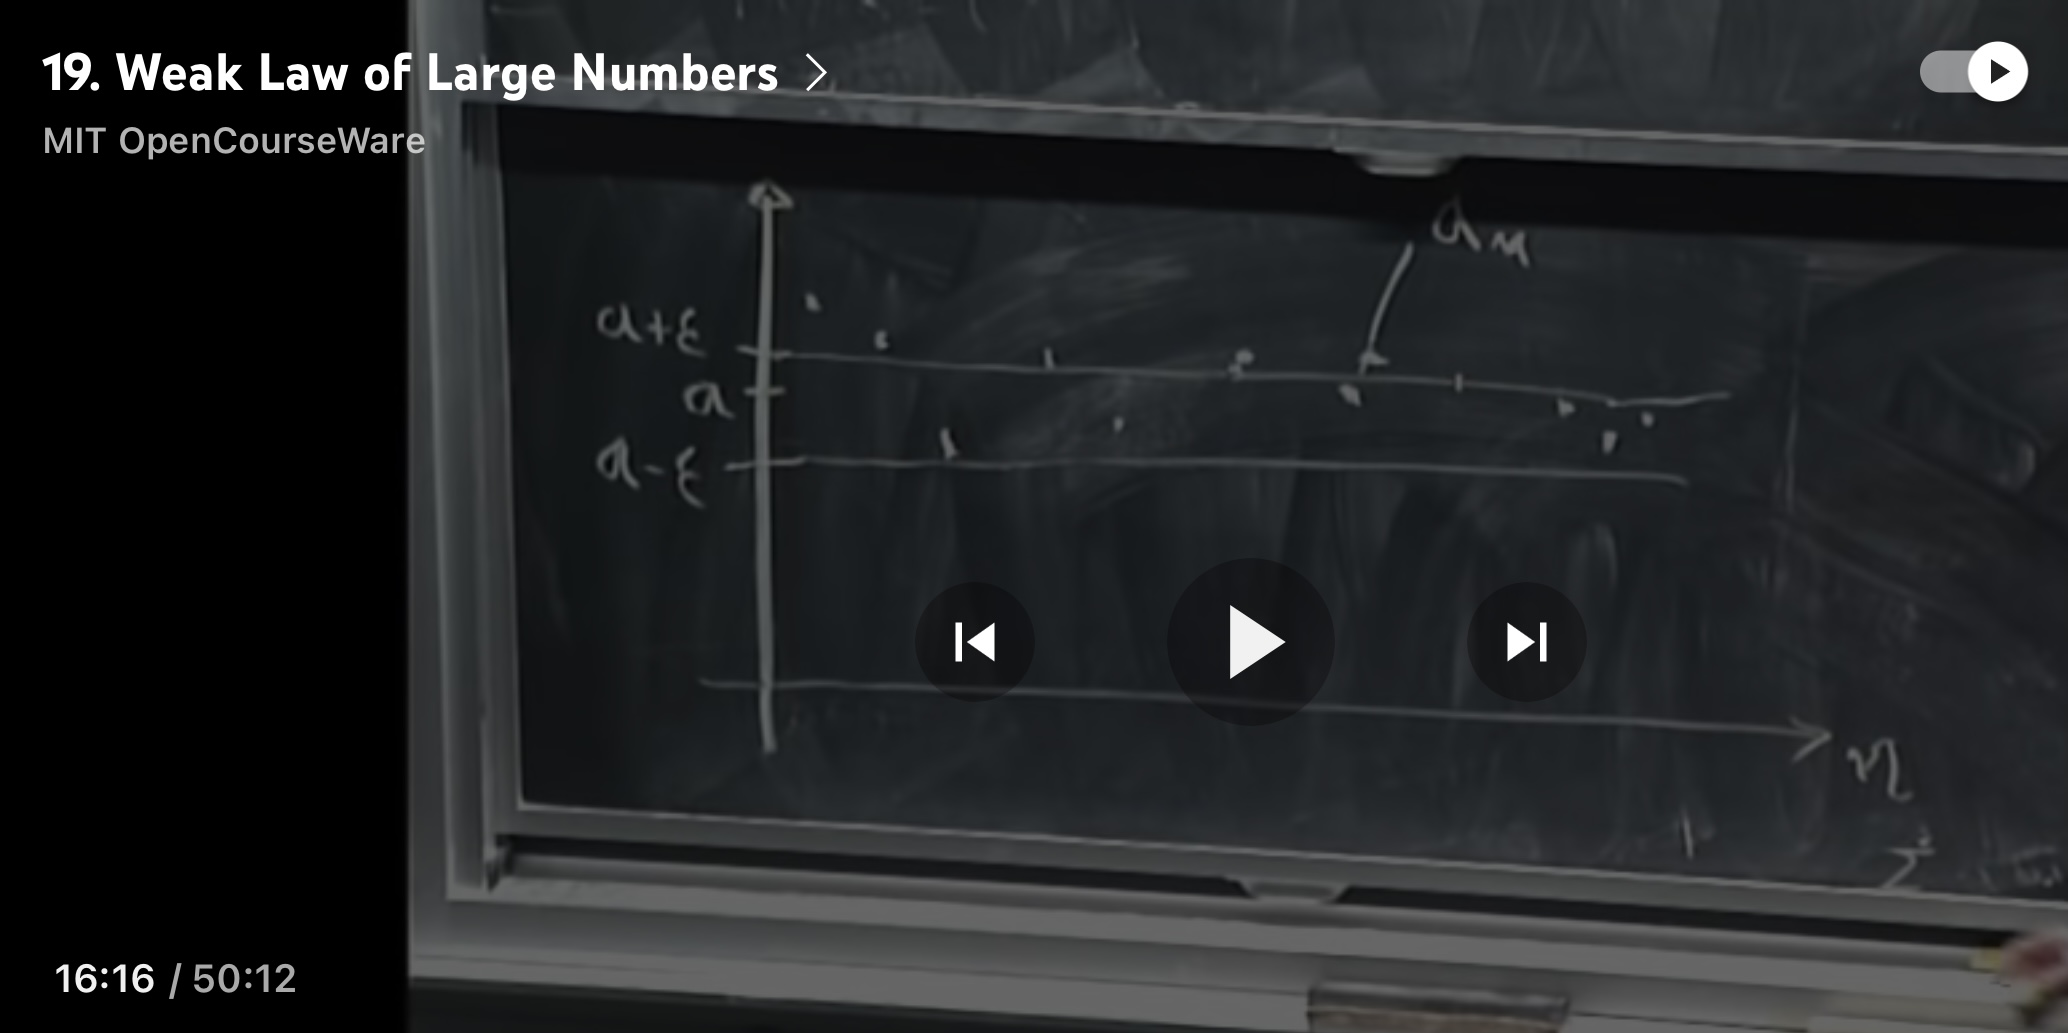
\includegraphics[width=7cm, height=4cm]{images/L19/IMG_3316.jpeg}
\caption{Convergence of a Sequence}
\end{figure}

\marginnote{\href{https://youtu.be/3eiio3Tw7UQ?16m20s}{(16:20)}}Convergence means given a band of positive length around the number a, the values of the sequence that you get, eventually stay inside the band.  This holds no matter how narrow the band is made to be.

\subsection{Convergence "in probability"}

\marginnote{\href{https://youtu.be/3eiio3Tw7UQ?17m50s}{(17:50)}}
\marginnote{Slide: Convergence "in probability"}

What does it mean for a sequence of random variables to converge to a number?

\marginnote{\href{https://youtu.be/3eiio3Tw7UQ?18m30s}{(18:30)}} Now we want the distribution inside the band.  The tails won't be, but we want more and more.

\begin{figure}[ht]
\centering
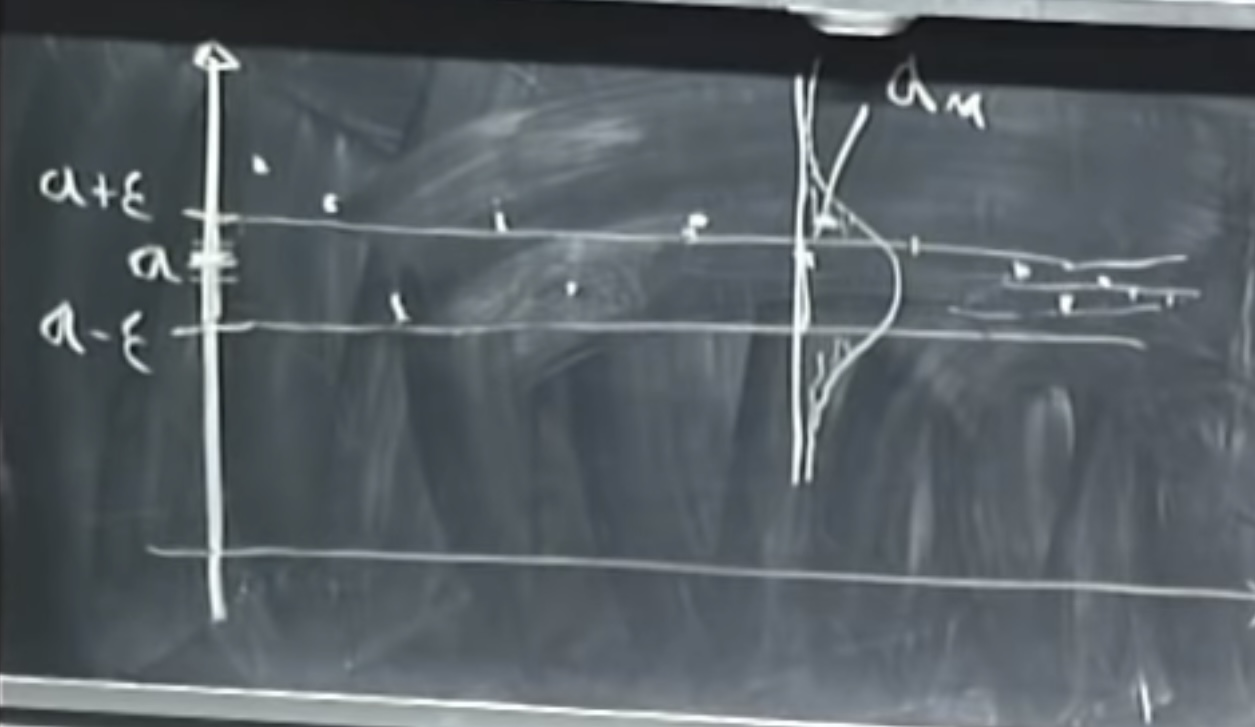
\includegraphics[width=7cm, height=4cm]{images/L19/IMG_3317.jpeg}
\caption{Convergence of RV}
\end{figure}

The mathematical statement is messy...better to think of the bands analogy.

\subsubsection*{Example}

\marginnote{\href{https://youtu.be/3eiio3Tw7UQ?22m00s}{(22:00)}}

\begin{figure}[ht]
\centering
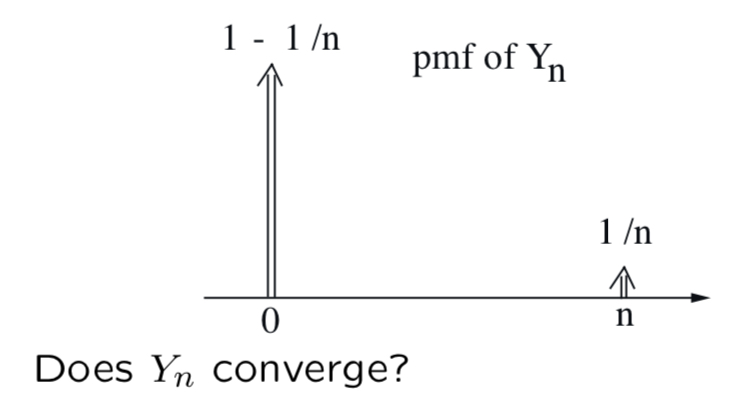
\includegraphics[width=7cm, height=4cm]{images/L19/IMG_1572.jpeg}
\caption{Does $Y_n converge?$}
\end{figure}

$Y_n$ converges in probability to zero.
What is the $\mathbb{E}[Y_n]$

\begin{align*}
    \mathbb{E}[Y_n] = n\cdot\frac{1}{n} = 1
\end{align*}

\begin{align*}
    \mathbb{E}[Y_n^2] = \infty
\end{align*}

\marginnote{\href{https://youtu.be/3eiio3Tw7UQ?24m00s}{(24:00)}} Convergences of a RV to zero doesn't imply anything about  convergence expected value, variance, etc.  It doesn't tell us how far the tail goes.

\subsection{Convergence of the Sample Mean}

\marginnote{\href{https://youtu.be/3eiio3Tw7UQ?25m00s}{(25:00 - Slide)}}

\begin{align*}
    M_n = \frac{X_1 + \cdots + X_n}{n} = \text{Sample Mean}
\end{align*}

\begin{align*}
    \mathbb{E}[M_n] = \frac{E[X_1] + \cdots + E[X_n]}{n} = \frac{n \mu}{n} = \mu
\end{align*}

\marginnote{\href{https://youtu.be/3eiio3Tw7UQ?27m00s}{(27:00)}} The sample mean is the heights we collected over a single expedition; this is $M_n$.  The expected value means thinking over a huge number of expeditions.  We average the averages at each expedition: $E[M_n]$.  Remember expectations always give numbers, where as the sample mean is a random variable.

\begin{align*}
    Var(M_n) = \frac{n \cdots \sigma^2}{n^2} = \frac{\sigma^2}{n}
\end{align*}
The variance of the sample mean becomes smaller and smaller.

Having a large sample size removes the randomness from the experiment.

Let's apply the Chebyshev inequality to say something about the tail probabilities for the sample mean.

The probability that you are more than $\varepsilon$ away from the true mean is less than or equal to $Var(M_n)/\varepsilon^2$:

\begin{align}
    P(|M_n - \mu| \ge \varepsilon) \le \frac{Var(M_n}{\varepsilon^2} = \frac{\sigma^2}{n \varepsilon^2}
\end{align}

We have convergence \emph{in probability} to the sample mean to the true mean.

\subsection{Example: The Pollster’s Problem}

\marginnote{\href{https://youtu.be/3eiio3Tw7UQ?30m45s}{(30:45)}}

Slide: The pollster’s problem\\

\marginnote{\href{https://youtu.be/3eiio3Tw7UQ?36m30s}{(36:30)}}
\begin{figure}[ht]
\centering
\includegraphics[width=7cm, height=4cm]{images/L19/IMG_3318.png}
\caption{$p(1-p)$}
\end{figure}

We are going to use the worst value for $\sigma_X^2$, which is 4.

Solving for n, we find that it needs to be greater than or equal to 50,000.

\marginnote{\href{https://youtu.be/3eiio3Tw7UQ?38m40s}{(38:40)}}

50,000 is too many people to sample so we try to cut corners.  Newspapers will go with $\pm$3 percentage points instead of 1 point.  This saves you a factor of 10.  Chebyshev is not a very tight inequality.  It's not that accurate.

\subsection{Different scalings of \texorpdfstring{$M_n$}{M}}

\marginnote{\href{https://youtu.be/3eiio3Tw7UQ?40m00s}{40:00)}}

Slide: Different scalings of $M_n$

\begin{figure}[ht]
\centering
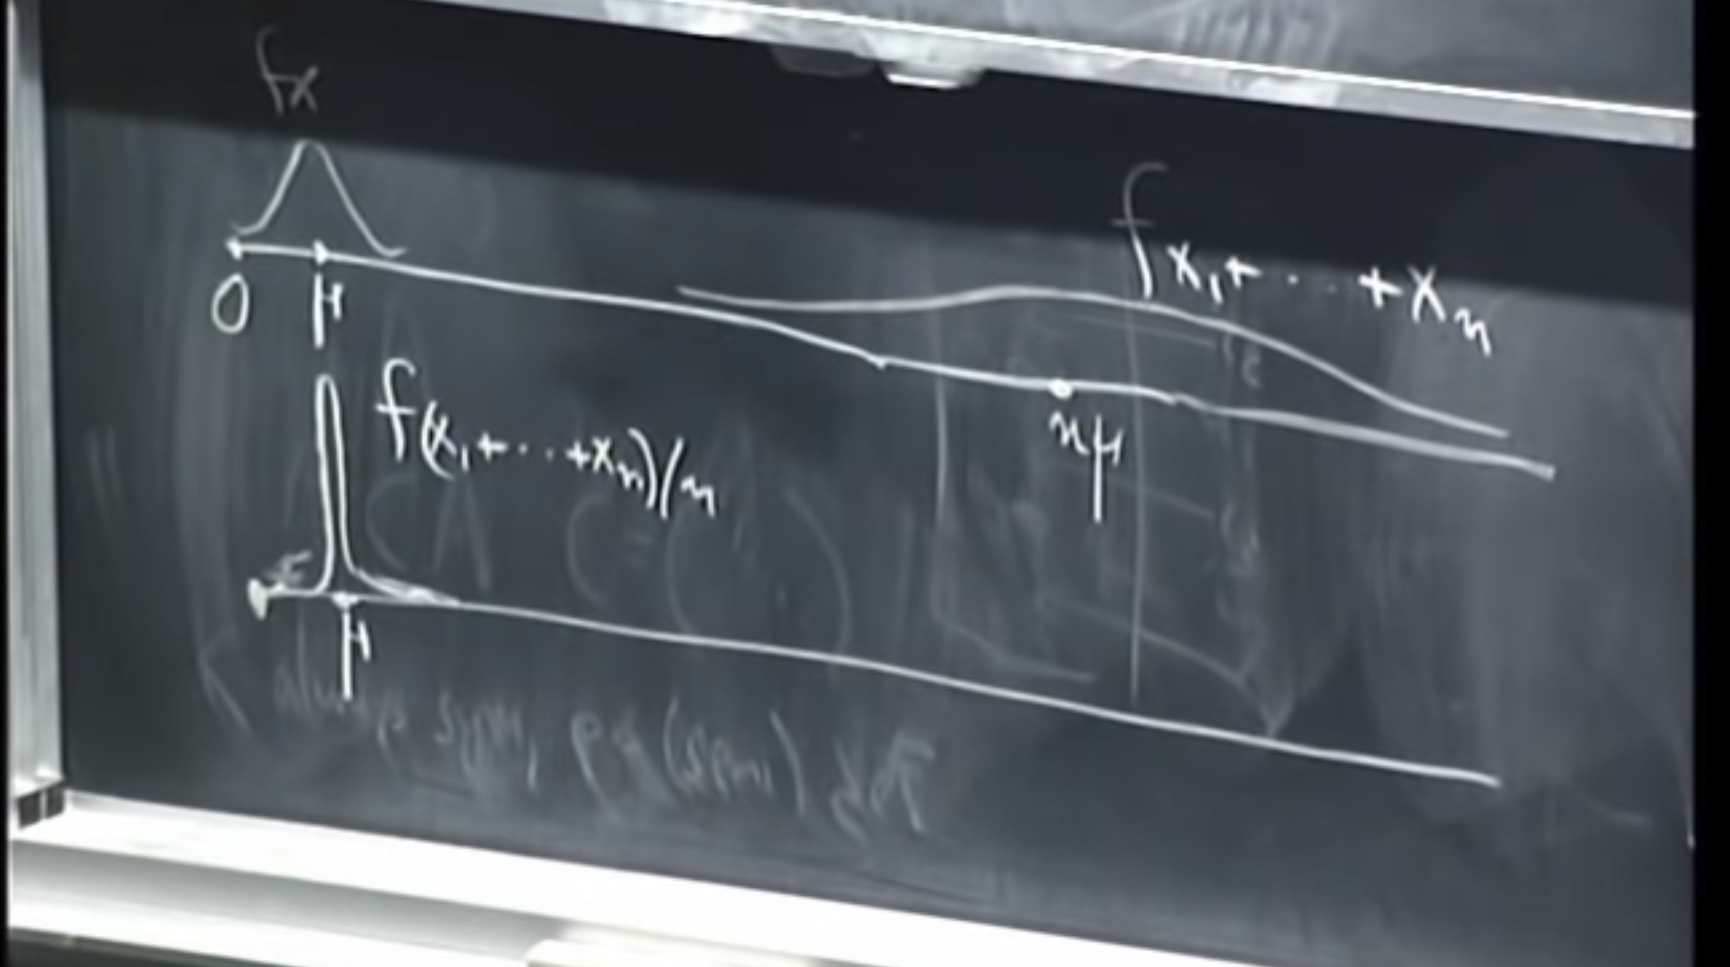
\includegraphics[width=7cm, height=4cm]{images/L19/IMG_3319.jpeg}
\caption{Scaling vs No Scaling}
\end{figure}

We decide to divide the sum by $\sqrt{n}$ instead of n.

\begin{figure}[ht]
\centering
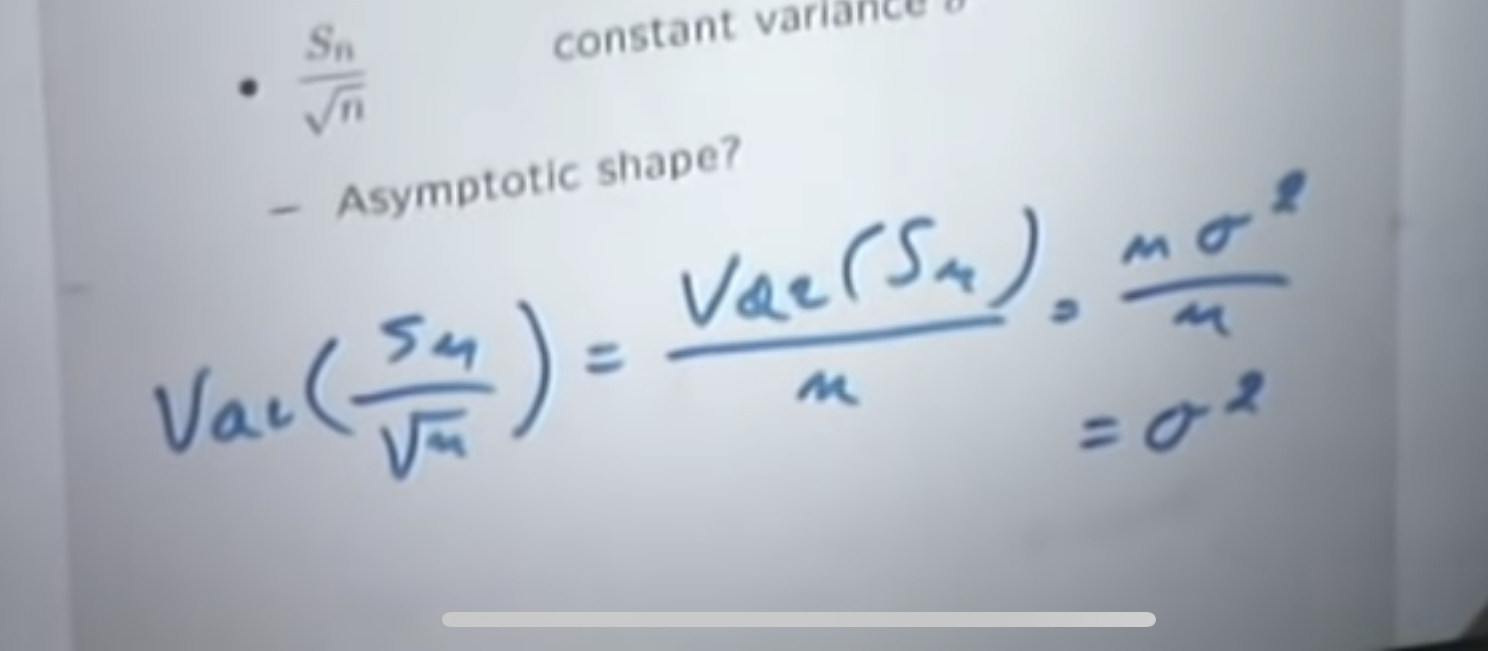
\includegraphics[width=7cm, height=4cm]{images/L19/IMG_3320.jpeg}
\caption{Eqn}
\end{figure}

\begin{align}
    Var(\frac{S_n}{\sqrt{n}})=\frac{Var(S_n)}{n} = \frac{n \sigma^2}{n} = \sigma^2
\end{align}

So, when we scale in this particular way $S_n$ changes but the variance doesn't change.

\subsection{Central Limit Theorem}

\marginnote{\href{https://youtu.be/3eiio3Tw7UQ?38m40s}{(44:10)}}

Slide: Central Limit Theorem\\

